\documentclass{standalone}
\usepackage{tikz}
\usetikzlibrary{patterns, positioning}
\usepackage[sfdefault]{ClearSans} %% option 'sfdefault' activates Clear Sans as the default text font
\usepackage[T1]{fontenc}

\begin{document}
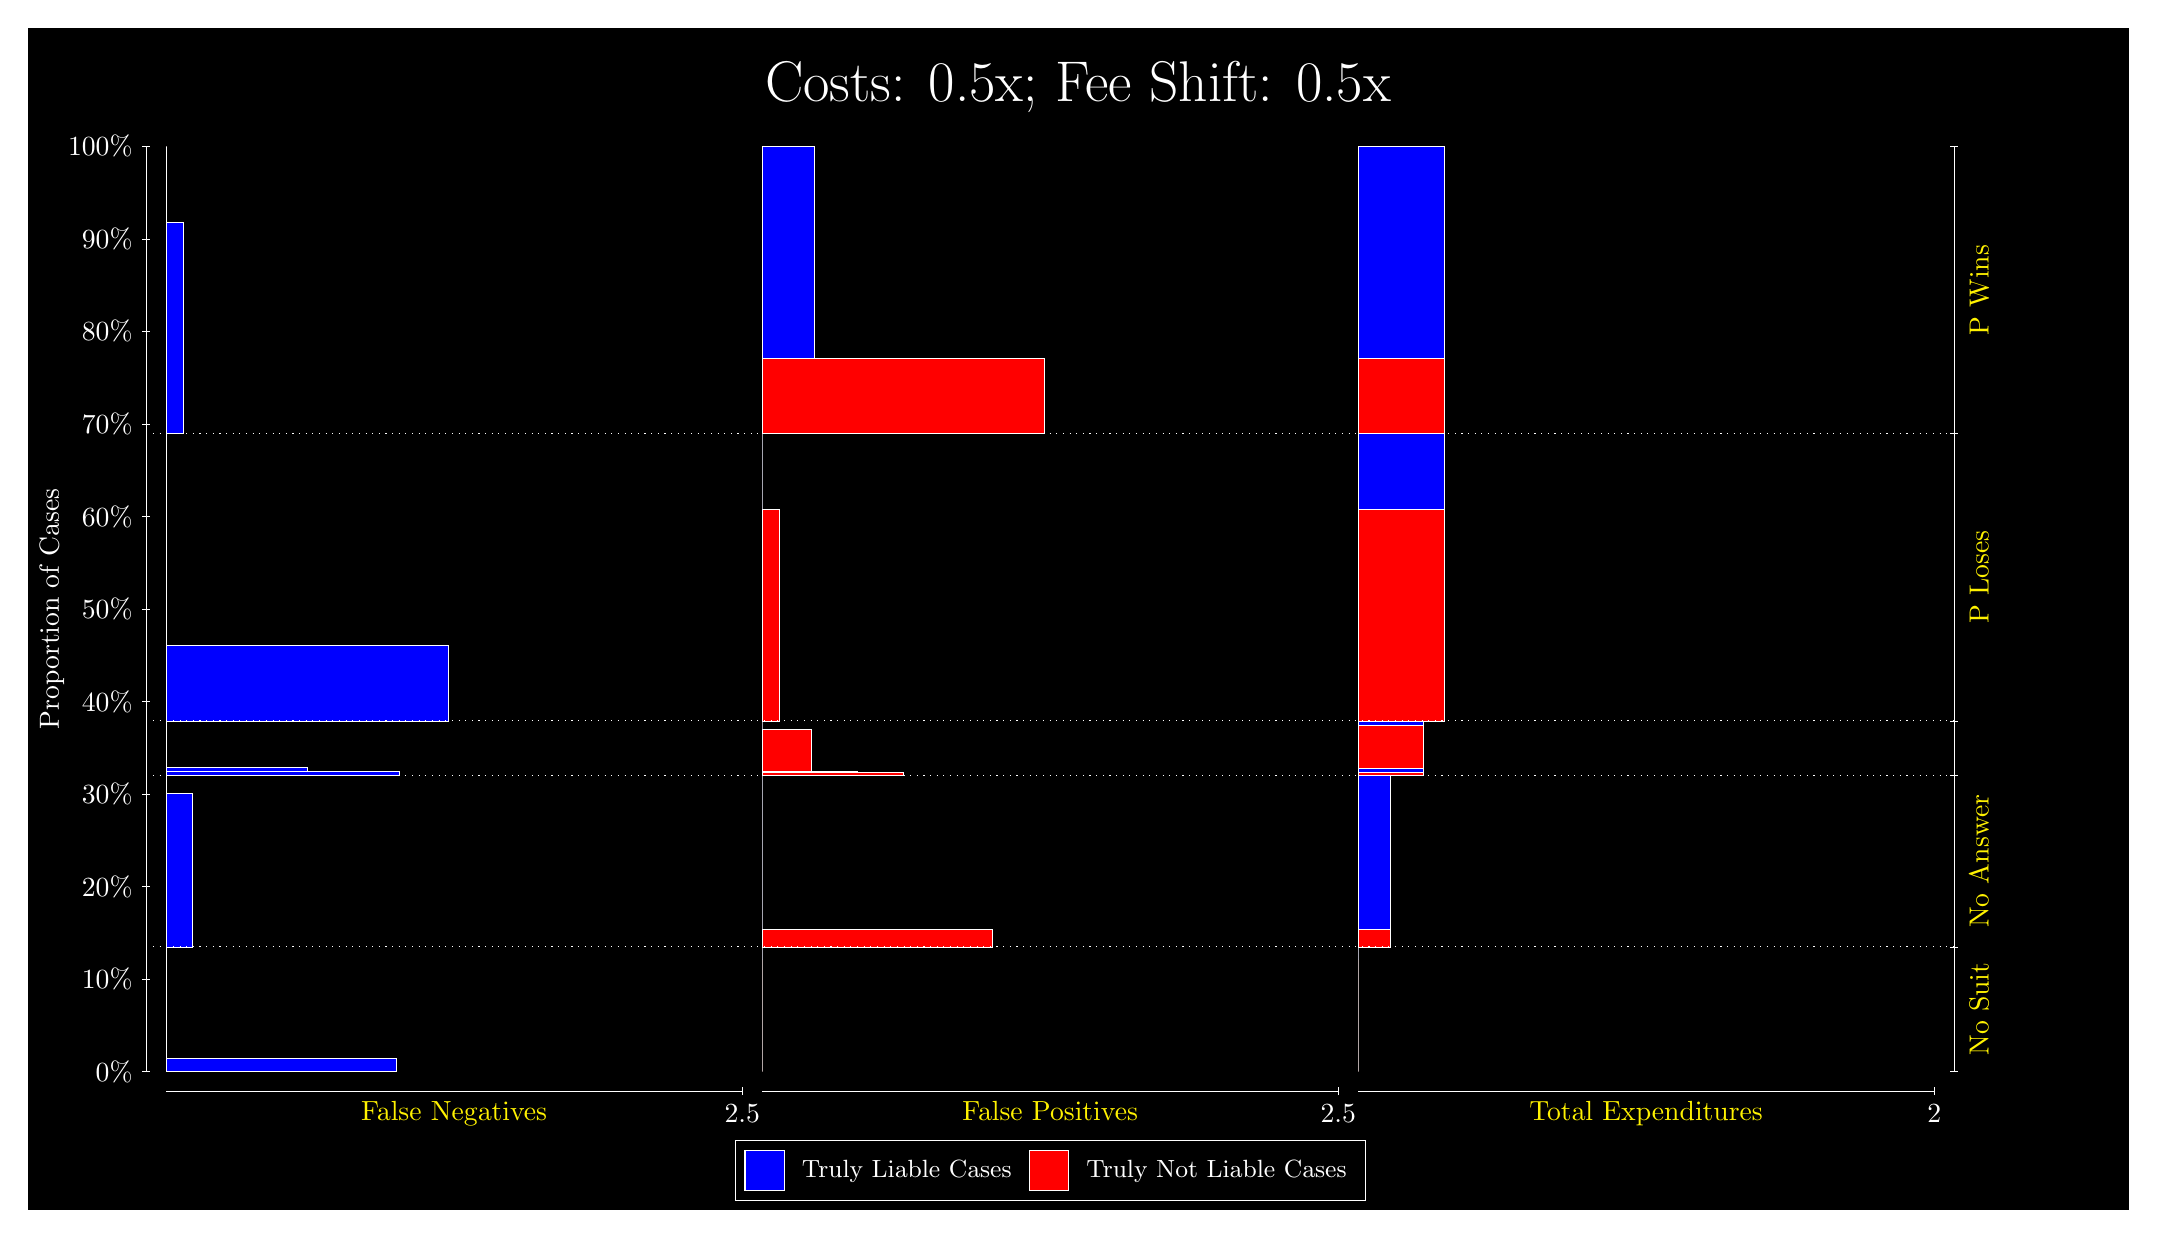
\begin{tikzpicture}
\draw[fill=black] (0,0) rectangle (26.667,15);
\draw[text=white] (0,13.5) rectangle (26.667,15) node[midway] {\huge Costs: 0.5x; Fee Shift: 0.5x};
\draw[white, very thin] (1.5,1.75) -- (1.5,13.5);
\node[rotate=90, text=white, anchor=center] at (0.3, 7.625) {Proportion of Cases};
\draw[white, very thin] (1.45,1.75) -- (1.55,1.75);
\node[text=white, anchor=east] at (1.45, 1.75) {0\%};
\draw[white, very thin] (1.45,2.925) -- (1.55,2.925);
\node[text=white, anchor=east] at (1.45, 2.925) {10\%};
\draw[white, very thin] (1.45,4.1) -- (1.55,4.1);
\node[text=white, anchor=east] at (1.45, 4.1) {20\%};
\draw[white, very thin] (1.45,5.275) -- (1.55,5.275);
\node[text=white, anchor=east] at (1.45, 5.275) {30\%};
\draw[white, very thin] (1.45,6.45) -- (1.55,6.45);
\node[text=white, anchor=east] at (1.45, 6.45) {40\%};
\draw[white, very thin] (1.45,7.625) -- (1.55,7.625);
\node[text=white, anchor=east] at (1.45, 7.625) {50\%};
\draw[white, very thin] (1.45,8.8) -- (1.55,8.8);
\node[text=white, anchor=east] at (1.45, 8.8) {60\%};
\draw[white, very thin] (1.45,9.975) -- (1.55,9.975);
\node[text=white, anchor=east] at (1.45, 9.975) {70\%};
\draw[white, very thin] (1.45,11.15) -- (1.55,11.15);
\node[text=white, anchor=east] at (1.45, 11.15) {80\%};
\draw[white, very thin] (1.45,12.325) -- (1.55,12.325);
\node[text=white, anchor=east] at (1.45, 12.325) {90\%};
\draw[white, very thin] (1.45,13.5) -- (1.55,13.5);
\node[text=white, anchor=east] at (1.45, 13.5) {100\%};

\draw[white, very thin] (24.457,1.75) -- (24.457,13.5);
\draw[white, very thin] (24.407,1.75) -- (24.507,1.75);
\node[anchor=west] at (24.407, 1.75) {};
\draw[white, very thin] (24.407,3.3335) -- (24.507,3.3335);
\node[anchor=west] at (24.407, 3.3335) {};
\draw[white, very thin] (24.407,5.5082) -- (24.507,5.5082);
\node[anchor=west] at (24.407, 5.5082) {};
\draw[white, very thin] (24.407,6.2032) -- (24.507,6.2032);
\node[anchor=west] at (24.407, 6.2032) {};
\draw[white, very thin] (24.407,9.8516) -- (24.507,9.8516);
\node[anchor=west] at (24.407, 9.8516) {};
\draw[white, very thin] (24.407,13.5) -- (24.507,13.5);
\node[anchor=west] at (24.407, 13.5) {};

\draw[white, very thin, fill=blue] (1.75,1.75) rectangle (4.6775,1.9166);
\draw[white, very thin, fill=red] (1.75,1.9166) rectangle (1.75,3.3335);
\draw[white, very thin, fill=blue] (1.75,3.3335) rectangle (2.0793,5.284);
\draw[white, very thin, fill=red] (1.75,5.284) rectangle (1.75,5.5082);
\draw[white, very thin, fill=blue] (1.75,5.5082) rectangle (4.7141,5.5638);
\draw[white, very thin, fill=blue] (1.75,5.5638) rectangle (4.1286,5.5695);
\draw[white, very thin, fill=blue] (1.75,5.5695) rectangle (3.5431,5.6177);
\draw[white, very thin, fill=red] (1.75,5.6177) rectangle (1.75,6.2032);
\draw[white, very thin, fill=blue] (1.75,6.2032) rectangle (5.3362,7.1652);
\draw[white, very thin, fill=red] (1.75,7.1652) rectangle (1.75,9.8516);
\draw[white, very thin, fill=blue] (1.75,9.8516) rectangle (1.9696,12.538);
\draw[white, very thin, fill=red] (1.75,12.538) rectangle (1.75,13.5);
\draw[white, very thin, fill=red] (9.3189,1.75) rectangle (9.3189,3.1669);
\draw[white, very thin, fill=blue] (9.3189,3.1669) rectangle (9.3189,3.3335);
\draw[white, very thin, fill=red] (9.3189,3.3335) rectangle (12.246,3.5578);
\draw[white, very thin, fill=blue] (9.3189,3.5578) rectangle (9.3189,5.5082);
\draw[white, very thin, fill=red] (9.3189,5.5082) rectangle (11.112,5.5565);
\draw[white, very thin, fill=red] (9.3189,5.5565) rectangle (10.526,5.5689);
\draw[white, very thin, fill=red] (9.3189,5.5689) rectangle (9.941,6.0937);
\draw[white, very thin, fill=blue] (9.3189,6.0937) rectangle (9.3189,6.2032);
\draw[white, very thin, fill=red] (9.3189,6.2032) rectangle (9.5384,8.8896);
\draw[white, very thin, fill=blue] (9.3189,8.8896) rectangle (9.3189,9.8516);
\draw[white, very thin, fill=red] (9.3189,9.8516) rectangle (12.905,10.814);
\draw[white, very thin, fill=blue] (9.3189,10.814) rectangle (9.9776,13.5);
\draw[white, very thin, fill=red] (16.888,1.75) rectangle (16.888,3.1669);
\draw[white, very thin, fill=blue] (16.888,3.1669) rectangle (16.888,3.3335);
\draw[white, very thin, fill=red] (16.888,3.3335) rectangle (17.299,3.5578);
\draw[white, very thin, fill=blue] (16.888,3.5578) rectangle (17.299,5.5082);
\draw[white, very thin, fill=red] (16.888,5.5082) rectangle (17.711,5.5565);
\draw[white, very thin, fill=blue] (16.888,5.5565) rectangle (17.711,5.6047);
\draw[white, very thin, fill=red] (16.888,5.6047) rectangle (17.711,6.142);
\draw[white, very thin, fill=blue] (16.888,6.142) rectangle (17.711,6.2032);
\draw[white, very thin, fill=red] (16.888,6.2032) rectangle (17.986,8.8896);
\draw[white, very thin, fill=blue] (16.888,8.8896) rectangle (17.986,9.8516);
\draw[white, very thin, fill=red] (16.888,9.8516) rectangle (17.986,10.814);
\draw[white, very thin, fill=blue] (16.888,10.814) rectangle (17.986,13.5);
\draw[white, dotted] (1.5,3.3335) -- (24.457,3.3335);
\draw[white, dotted] (1.5,5.5082) -- (24.457,5.5082);
\draw[white, dotted] (1.5,6.2032) -- (24.457,6.2032);
\draw[white, dotted] (1.5,9.8516) -- (24.457,9.8516);
\draw[white, very thin] (1.75,1.5) -- (9.0689,1.5);
\node[text=yellow, anchor=north] at (5.4094, 1.5) {False Negatives};
\draw[white, very thin] (9.0689,1.45) -- (9.0689,1.55);
\node[text=white, anchor=north] at (9.0689, 1.45) {2.5};

\draw[white, very thin] (9.3189,1.5) -- (16.638,1.5);
\node[text=yellow, anchor=north] at (12.978, 1.5) {False Positives};
\draw[white, very thin] (16.638,1.45) -- (16.638,1.55);
\node[text=white, anchor=north] at (16.638, 1.45) {2.5};

\draw[white, very thin] (16.888,1.5) -- (24.207,1.5);
\node[text=yellow, anchor=north] at (20.547, 1.5) {Total Expenditures};
\draw[white, very thin] (24.207,1.45) -- (24.207,1.55);
\node[text=white, anchor=north] at (24.207, 1.45) {2};

\node[text=yellow, centered, rotate=90] at (24.777, 2.5418) {No Suit};
\node[text=yellow, centered, rotate=90] at (24.777, 4.4209) {No Answer};

\node[text=yellow, centered, rotate=90] at (24.777, 8.0274) {P Loses};
\node[text=yellow, centered, rotate=90] at (24.777, 11.676) {P Wins};

\draw (12.978300999999998,1.5) node[draw=none] (baseCoordinate) {};
\begin{scope}[align=center]
        \matrix[scale=0.5, draw=white, below=0.5cm of baseCoordinate, nodes={draw}, column sep=0.1cm]{
            \node[rectangle, draw, minimum width=0.5cm, minimum height=0.5cm, fill=blue] {}; &
            \node[draw=none, font=\small, text=white] (B) {Truly Liable Cases}; &
            \node[rectangle, draw, minimum width=0.5cm, minimum height=0.5cm, fill=red] {}; &
            \node[draw=none, font=\small, text=white] (B) {Truly Not Liable Cases}; \\
            };
\end{scope}

\end{tikzpicture}
\end{document}